\documentclass[]{elsarticle} %review=doublespace preprint=single 5p=2 column
%%% Begin My package additions %%%%%%%%%%%%%%%%%%%
\usepackage[hyphens]{url}

  \journal{Astronomy \& Astrophysics} % Sets Journal name


\usepackage{lineno} % add
\providecommand{\tightlist}{%
  \setlength{\itemsep}{0pt}\setlength{\parskip}{0pt}}

\bibliographystyle{elsarticle-harv}
\biboptions{sort&compress} % For natbib
\usepackage{graphicx}
\usepackage{booktabs} % book-quality tables
%%%%%%%%%%%%%%%% end my additions to header

\usepackage[T1]{fontenc}
\usepackage{lmodern}
\usepackage{amssymb,amsmath}
\usepackage{ifxetex,ifluatex}
\usepackage{fixltx2e} % provides \textsubscript
% use upquote if available, for straight quotes in verbatim environments
\IfFileExists{upquote.sty}{\usepackage{upquote}}{}
\ifnum 0\ifxetex 1\fi\ifluatex 1\fi=0 % if pdftex
  \usepackage[utf8]{inputenc}
\else % if luatex or xelatex
  \usepackage{fontspec}
  \ifxetex
    \usepackage{xltxtra,xunicode}
  \fi
  \defaultfontfeatures{Mapping=tex-text,Scale=MatchLowercase}
  \newcommand{\euro}{€}
\fi
% use microtype if available
\IfFileExists{microtype.sty}{\usepackage{microtype}}{}
\usepackage[left=4cm, right=3cm, top=2.5cm, bottom=2.5cm]{geometry}
\usepackage{graphicx}
% We will generate all images so they have a width \maxwidth. This means
% that they will get their normal width if they fit onto the page, but
% are scaled down if they would overflow the margins.
\makeatletter
\def\maxwidth{\ifdim\Gin@nat@width>\linewidth\linewidth
\else\Gin@nat@width\fi}
\makeatother
\let\Oldincludegraphics\includegraphics
\renewcommand{\includegraphics}[1]{\Oldincludegraphics[width=\maxwidth]{#1}}
\ifxetex
  \usepackage[setpagesize=false, % page size defined by xetex
              unicode=false, % unicode breaks when used with xetex
              xetex]{hyperref}
\else
  \usepackage[unicode=true]{hyperref}
\fi
\hypersetup{breaklinks=true,
            bookmarks=true,
            pdfauthor={},
            pdftitle={The Locus Algorithm},
            colorlinks=false,
            urlcolor=blue,
            linkcolor=magenta,
            pdfborder={0 0 0}}
\urlstyle{same}  % don't use monospace font for urls

\setcounter{secnumdepth}{0}
% Pandoc toggle for numbering sections (defaults to be off)
\setcounter{secnumdepth}{0}
% Pandoc header
\usepackage{booktabs}
\usepackage{longtable}
\usepackage{array}
\usepackage{multirow}
\usepackage{wrapfig}
\usepackage{float}
\usepackage{colortbl}
\usepackage{pdflscape}
\usepackage{tabu}
\usepackage{threeparttable}
\usepackage{threeparttablex}
\usepackage[normalem]{ulem}
\usepackage{makecell}
\usepackage{xcolor}
\usepackage{commath}
\usepackage{amsmath}



\begin{document}
\begin{frontmatter}

  \title{The Locus Algorithm}
    \author[Dublin Institute for Advanced Studies]{O. Creaner\corref{c1}}
   \ead{creanero@cp.dias.ie} 
   \cortext[c1]{Corresponding Author}
    \author[Technological University Dublin]{E. Hickey}
   \ead{eugene.hickey@it-tallaght.ie} 
  
    \author[Technological University Dublin]{K.Nolan}
   \ead{kevin.nolan@it-tallaght.ie} 
  
    \author[Cork Institute of Technology]{N.Smith}
   \ead{nsmith@cit.ie} 
  
      \address[Dublin Institute for Advanced Studies]{Dublin Institute for Advanced Studies, 31 Fitzwilliam Place, Dublin 2,
Ireland}
    \address[Technological University Dublin]{Technological University Dublin, Tallaght Campus, Dublin 24, Ireland}
    \address[Cork Institute of Technology]{Cork Institute of Technology, Bishopstown, Cork, Ireland}
  
  \begin{abstract}
  We describe the design, implementation and operation of a new algorithm,
  The Locus Algorithm; which enables optimised differential photometry.
  For a given target, The Locus Algorithm identifies the pointing for
  which the resultant FoV includes the target and the maximum number of
  similar reference stars available, thus enabling optimised differential
  photometry of the target. We describe the application of The Locus
  Algorithm to a target from the Sloan Digital Sky Survey to provide
  optimum differential photometry for that target. The algorithm was also
  used to generate catalogues of pointing's to optimise Quasars
  variability studies and to generate catalogues of optimised pointings in
  the search for Exoplanets via the transit method.
  \end{abstract}
  
 \end{frontmatter}

\hypertarget{introduction}{%
\section{Introduction}\label{introduction}}

Photometric variability studies involve identifying variations in
brightness of a celestial point source over time. Such studies are
hampered by the Earth's atmosphere, which causes first order and second
order extinction Milone and Pel (2011) YOUNG et al. (1991). Differential
Photometry mitigates the effect of the Earth's atmosphere by comparing
the brightness of a target to reference stars in the same Field of View
(FoV). Differential photometry can be optimised for the target by
choosing a pointing whose Field of View (FoV) includes the target and
the maximum number of reference stars of similar magnitude and colour.
Milone and Pel (2011) YOUNG et al. (1991) Howell and B. (2000) Honeycutt
(1992).

The Locus Algorithm enables optimised differential photometry by
identifying the pointing for which the resultant FoV includes the target
and the best set of similar reference stars available.

\hypertarget{conceptual-basis-to-the-locus-algorithm}{%
\section{Conceptual basis to The Locus
Algorithm}\label{conceptual-basis-to-the-locus-algorithm}}

A locus can be defined around any star such that a FoV centred on any
point on the locus will include the star at the edge of the FoV. For
fields containing stars close to one another, if one locus intersects
with another, they produce Points of Intersection (PoIs) (Figure 1).

\begin{figure}
\centering
\includegraphics{fig1.png}
\caption{Figure 1. Diagrammatic representation of two stars with loci
(red and blue perimeter lines), which intersect and produce two Points
of Intersection (PoI's) circled in yellow.}
\end{figure}

A FoV centred on any such PoI will include both stars associated with
creating it. At Points of Intersection the set of stars that can be
included in a FoV changes.

The Locus Algorithm considers candidate reference stars in what is
termed a Candidate Zone (CZ) - the zone of sky centred on the target
within which a FoV can be selected which includes both the reference
star and the target. Within the Candidate Zone, all relevant Points of
Intersection are identified. Each PoI is assigned a score derived from
the number and similarity of reference stars included in it's resulting
FoV. The PoI with the highest score becomes the pointing for the target.

\hypertarget{locus-algorithm-design}{%
\section{Locus Algorithm Design}\label{locus-algorithm-design}}

\hypertarget{definition-of-coordinate-system-and-locus}{%
\subsection{Definition of Coordinate System and
Locus}\label{definition-of-coordinate-system-and-locus}}

For computational efficiency, The Locus Algorithm considers a Field of
View to be a rectangular area on the sky orientated such that the edges
are aligned with the primary x and y axes of the Cartesian coordinate
system. Movement of the field is restricted to x or y translations.

However, the Celestial coordinate system is defined by the Equatorial
coordinate system, with coordinates specified by Right Ascension (RA)
and Declination (Dec). Because this is a spherical coordinate system,
unit angle in RA is foreshortened, with the degree of foreshortening
defined by:

\[angle \in RA = {\frac{True Angle}{cosine(Dec)}} \tag{Equation 1: Right Ascension foreshortening with Declination}\]

By using this conversion, it is possible to approximate to a high degree
of accuracy a Cartesian coordinate system using RA and Dec; with a small
FoV of horizontal size R and vertical size S about a star located at
point \(RA_c\) and \(Dec_c\) , where

\[R^` = {\frac{R}{cos(Dec_c)}}\] as:

\[RA_c - {\frac{R^`}{2}} \leq RA \leq RA_c + {\frac{R^`}{2}} \]

\[Dec_c - {\frac{S}{2}} \leq Dec \leq Dec_c + {\frac{S}{2}}\]

Equation 2. Definition of a FoV of size R x S centred on a point
(\(RA_c\) , \(Dec_c\))

This definition is accurate to approximately 1\% for a FoV of area 15'
square outside celestial polar regions; and does not consider RA ``loop
around'' from 359.99\(^{\circ}\) to 0.00\(^{\circ}\); resulting, for
example, in the exclusion of 0.23\% of the SDSS catalogue. Planned
enhancements to The Locus Algorithm will resolve these shortcomings.

We can therefore define the locus about any star on the sky located at
\(RA_c\) and \(Dec_c\) as the values of Right Ascension and Declination
as defined in Equation 2.

\hypertarget{candidate-zone}{%
\subsection{Candidate Zone}\label{candidate-zone}}

A Candidate Zone is defined as a region centred on the target, equal to
four times the area of any Field of View (Equation 3), within which any
reference star can be included in a Field of View with the target and
can therefore be considered as a candidate reference star in identifying
the optimum pointing. Conversely, stars outside the candidate zone
cannot be included in a Field of View with the target and cannot
therefore be considered as candidates reference stars. Hence the
Candidate Zone is the maximum region of sky centred on the target from
which to choose candidate reference stars when identifying an optimum
pointing for a given target. For a target positioned at coordinates
\(RA_c\) and \(Dec_c\) the resulting Candidate Zone is defined by:

\[RA_c - R^` \leq RA \leq RA_c + R^` \]

\[Dec_c - S \leq Dec \leq Dec_c + S\]

Equation 3. Definition of a Candidate Zone of size 2R x 2S centred on a
target with coordinates (\(RA_c\), \(Dec_c\))

\begin{figure}
\centering
\includegraphics{fig2.png}
\caption{Figure 2. Modified image taken from the SDSS ``Navigate'' tool.
The image showing fields (in red) needed to form a mosaic from which a
Candidate Zone (green) centred on the target can be defined.}
\end{figure}

\hypertarget{identification-and-filtering-of-reference-stars}{%
\subsection{Identification and Filtering of Reference
Stars}\label{identification-and-filtering-of-reference-stars}}

For each target, a list of candidate reference stars in its Candidate
Zone is produced based on the following criteria:

\begin{itemize}
\tightlist
\item
  Position: the reference star must be in the Candidate Zone.
\item
  Magnitude: the reference star must be within a user-defined limit of
  the target's magnitude.
\item
  Colour: the reference star must match the colour of the target to
  within a user-specified limit.
\item
  Resolvability: the reference star must be resolvable, i.e.~no other
  star that would impact a brightness measurements within a
  user-specified resolution limit.
\end{itemize}

All stars in the Candidate Zone which pass these initial filters become
the list of candidate reference stars from which loci will be
identified.

\hypertarget{identifying-the-effective-locus-for-each-candidate-reference-star}{%
\subsection{Identifying the Effective Locus for each Candidate Reference
Star}\label{identifying-the-effective-locus-for-each-candidate-reference-star}}

The locus associated with each candidate reference star must be
identified based on Equation 2. For the purposes of identifying Points
of Intersection, only the side surrounding a given candidate reference
star closest to the target need be considered. Hence, we can define the
effective locus for such a candidate reference star as a single line of
constant RA and a single line of constant Dec nearest the target star
(Figure 3).

\begin{figure}
\centering
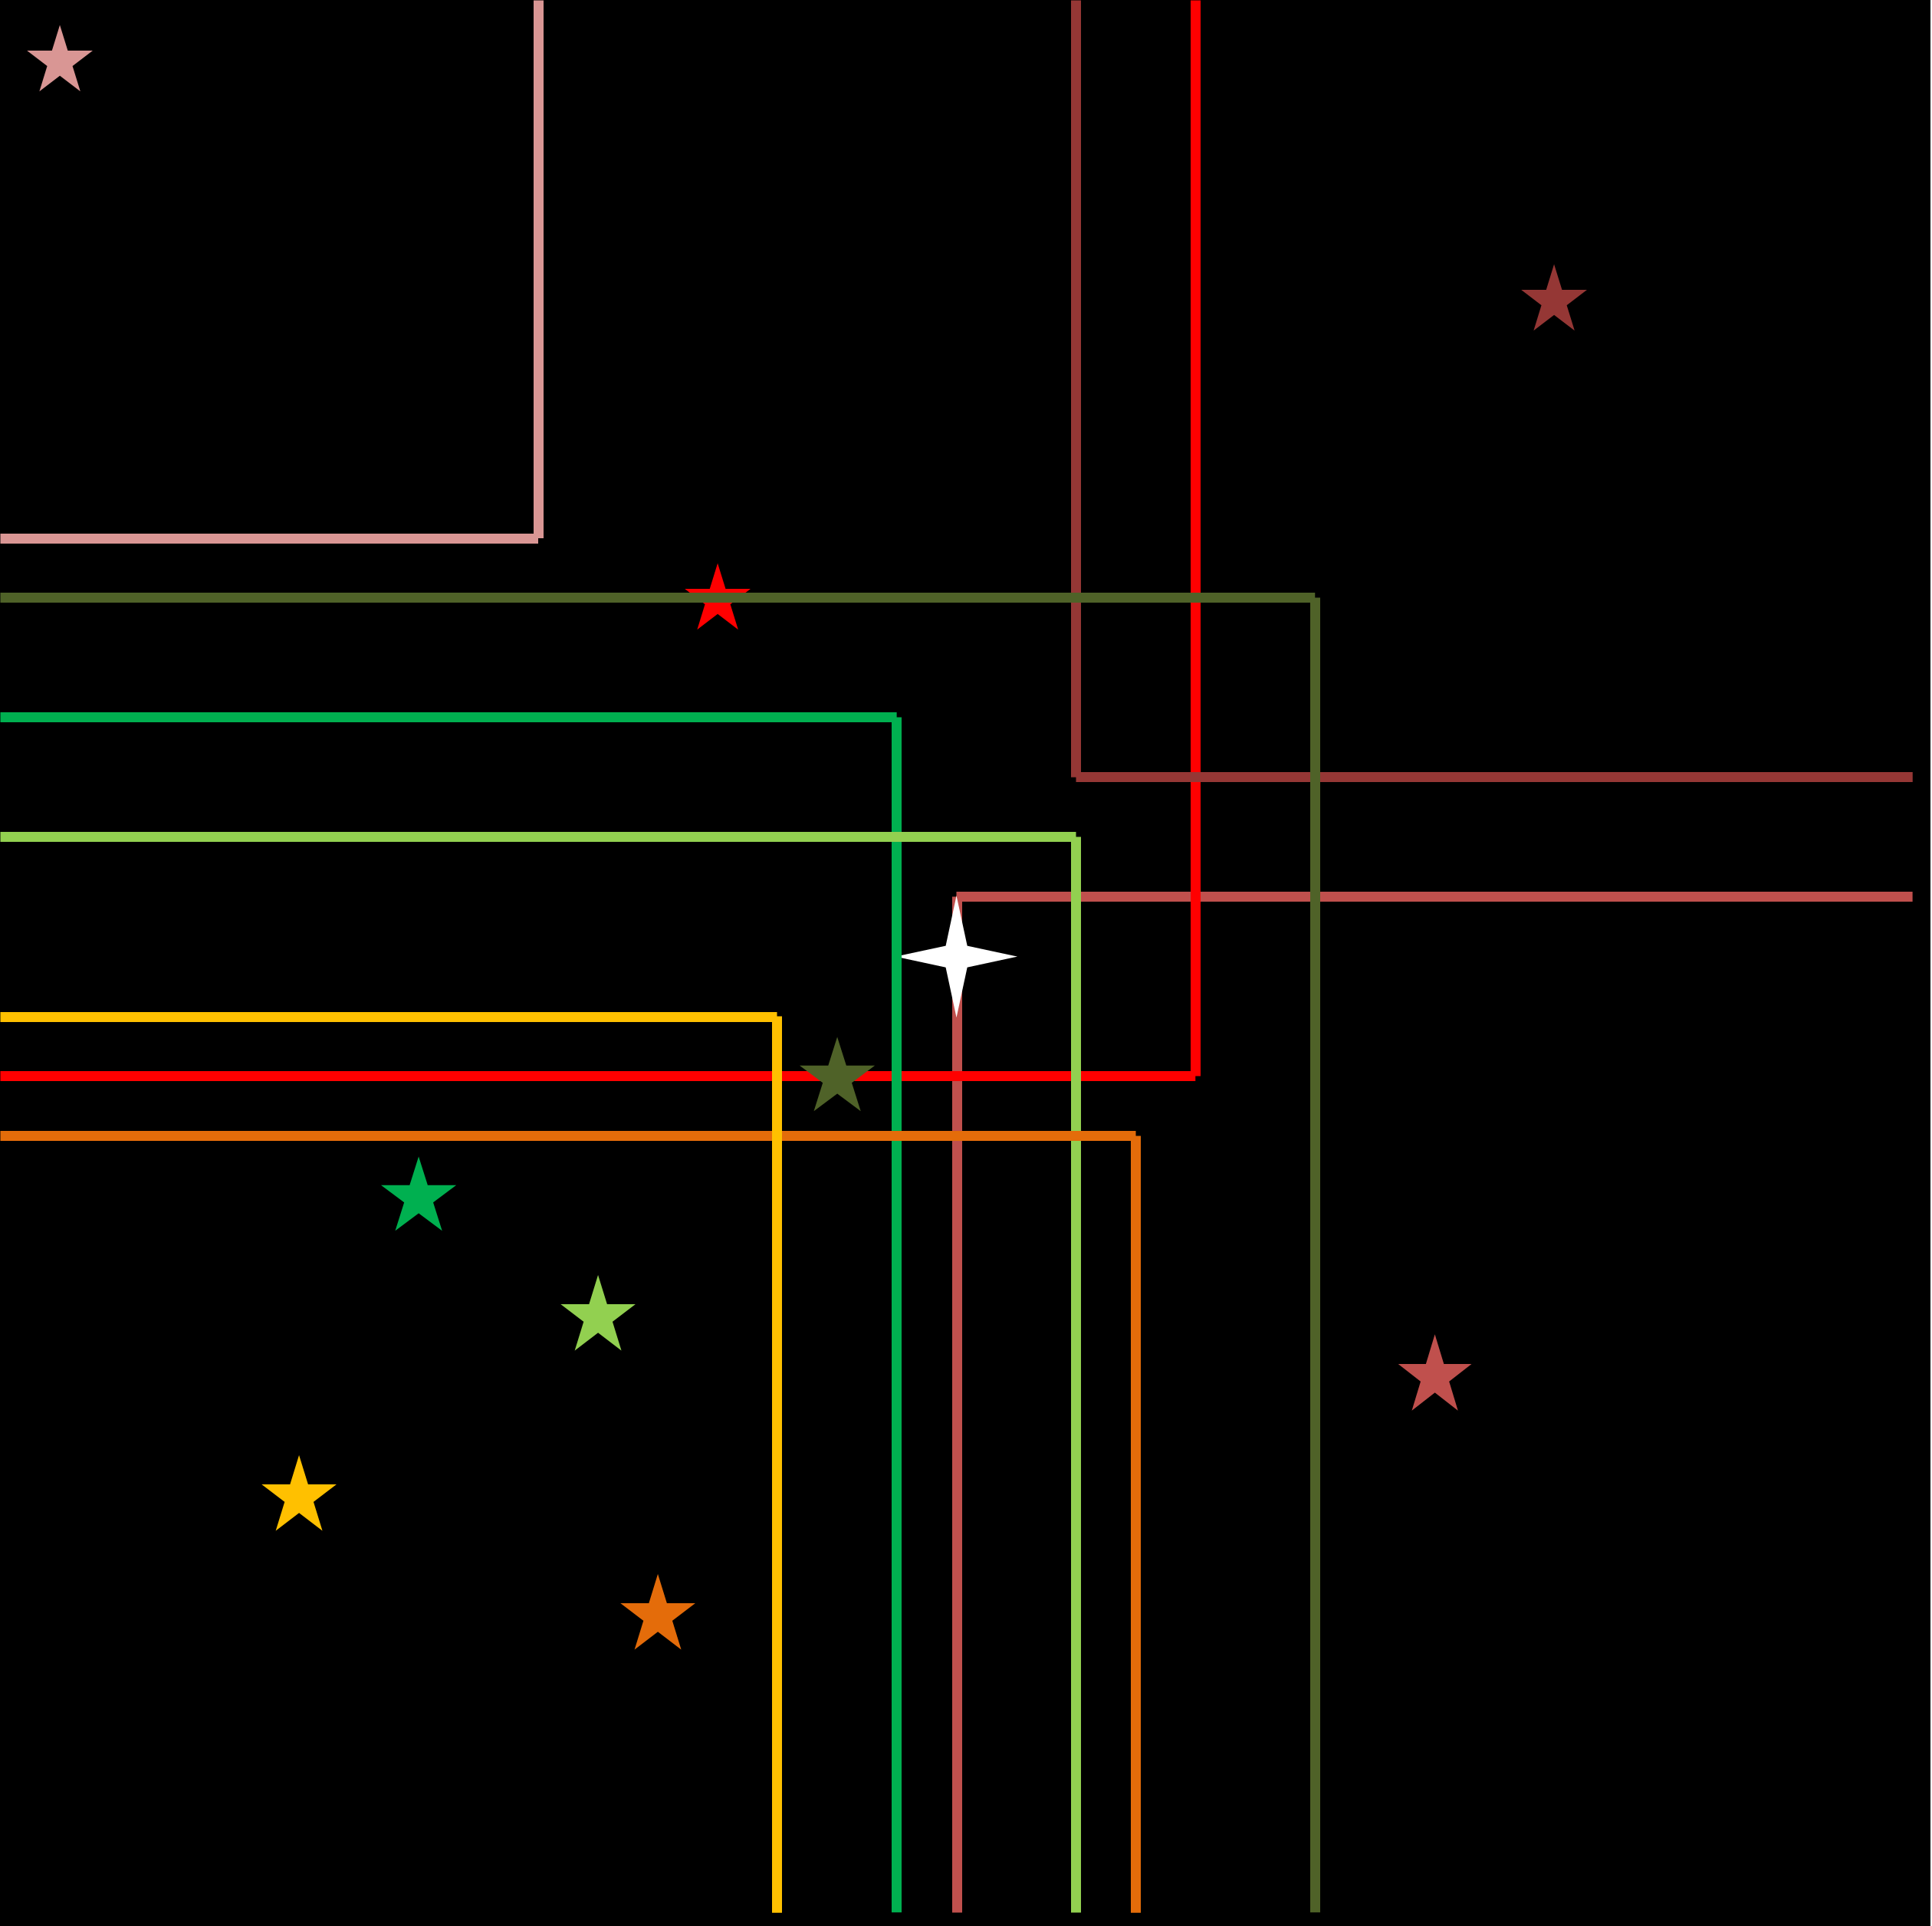
\includegraphics{fig3.png}
\caption{Figure 3: Each effective locus is defined by assigning a pair
of RA and Dec coordinates for a corner point and a pair of lines North
or South and East or West from the corner point. In this diagram, each
candidate reference star is assigned a colour, and the effective locus
that corresponds to it is drawn in the same colour.}
\end{figure}

Specifically, the effective locus can be defined as a corner point of
the locus and two lines: one of constant RA and the other of constant
Dec emanating from the corner point. The direction of the lines is
determined by the Right Ascension and Declination of the candidate
reference star relative to the target; as follows:

\begin{itemize}
\tightlist
\item
  If the RA of the candidate is greater than the target, the line of
  constant Dec is drawn in the direction of increasing RA
\item
  If the RA of the candidate is less than the target, the line of
  constant Dec is drawn in the direction of decreasing RA
\item
  If the Dec of the candidate is greater than the target, the line of
  constant RA is drawn in the direction of increasing Dec
\item
  If the Dec of the candidate is less than the target, the line of
  constant RA is drawn in the direction of decreasing Dec.
\end{itemize}

Using the Equatorial Coordinate System discussed in Section 3.1, with
coordinates of the target specified by \((RA_{target}, Dec_{target})\)
and coordinates of the candidate reference star defined by
\((RA_{reference}, Dec_{reference})\) and a size of FoV of horizontal
length R and vertical length S, the coordinates of the corner point
\((RA_{corner-point}, Dec_{corner-point})\) are defined as:

\[RA_{target} \leq RA_{reference} \Rightarrow RA_{corner-point} = RA_{reference}- R^` \]

\[RA_{target} > RA_{reference} \Rightarrow RA_{corner-point} = RA_{reference}+ R^` \]

\[Dec_{target} \leq Dec_{reference} \Rightarrow Dec_{corner-point} = Dec_{reference}- {\frac{S}{2}} \]

\[Dec_{target} > Dec_{reference} \Rightarrow Dec_{corner-point} = Dec_{reference} + {\frac{S}{2}}\]

The direction of the lines of constant RA and Dec of the effective locus
emanating from any such corner point are determined according to the
criteria describe above.

\hypertarget{identifying-and-scoring-points-of-intersection-and-identifying-the-pointing.}{%
\subsection{Identifying and Scoring Points of Intersection and
identifying the
pointing.}\label{identifying-and-scoring-points-of-intersection-and-identifying-the-pointing.}}

The points where lines from any two loci are identified. This involves
comparing the corner point RA and Dec and direction of lines for one
locus with the corner point RA and Dec and direction of lines for a
second locus. In total eight variable associated with each two loci are
checked:

\begin{itemize}
\tightlist
\item
  For Locus 1: \(RA_1\), \(Dec_1\), \(DirRA_1\), \(DirDec_1\)
\item
  For Locus 2: \(RA_2\), \(Dec_2\), \(DirRA_2\), \(DirDec_2\)
\end{itemize}

Using these parameters, a check as to whether an intersection between
the two loci occurs is achieved as follows:

\begin{itemize}
\tightlist
\item
  A line of constant Dec in the positive RA direction from the corner
  point of locus 1 will intersect with a line of constant RA in the
  positive Dec direction from the corner point of locus 2 if locus 1 has
  a lower RA than locus 2 and locus 1 has a higher Dec than locus 2.
\item
  A line of constant RA in the positive Dec direction from the corner
  point of locus 1 will intersect with a line of constant Dec in the
  positive RA direction from the corner point of locus 2 if locus 1 has
  a lower Dec than locus 2 and locus 1 has a higher RA than locus 2.
\end{itemize}

\ldots{} and so on. By checking all such possible combinations, all
pairs of loci in the field which result in a Point of Intersection are
identified and their RA and Dec noted.

Subsequent to identification, each Point of Intersection is then scored.
This is achieved as follows:

\begin{itemize}
\tightlist
\item
  The number of reference stars in the Field of View centred on the
  Point of Intersection is counted.
\item
  Each reference star is assigned a rating value between 0 and 1 based
  on its similarity in colour to the target.
\item
  The ratings from all counted reference stars in the Field of View are
  combined into one overall score for the field (Figure 4).
\item
  The Point of Intersection with the highest score becomes the pointing
  for the target (Figure 5).
\end{itemize}

\begin{figure}
\centering
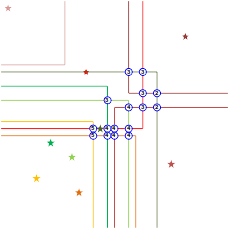
\includegraphics{fig4.png}
\caption{Figure 4. Points of Intersection (PoI), and their associated
score. In this diagram each star has a rating of 1, hence the score
associated with each PoI is equal to the number of reference stars
within a FoV centred at that PoI.}
\end{figure}

\begin{figure}
\centering
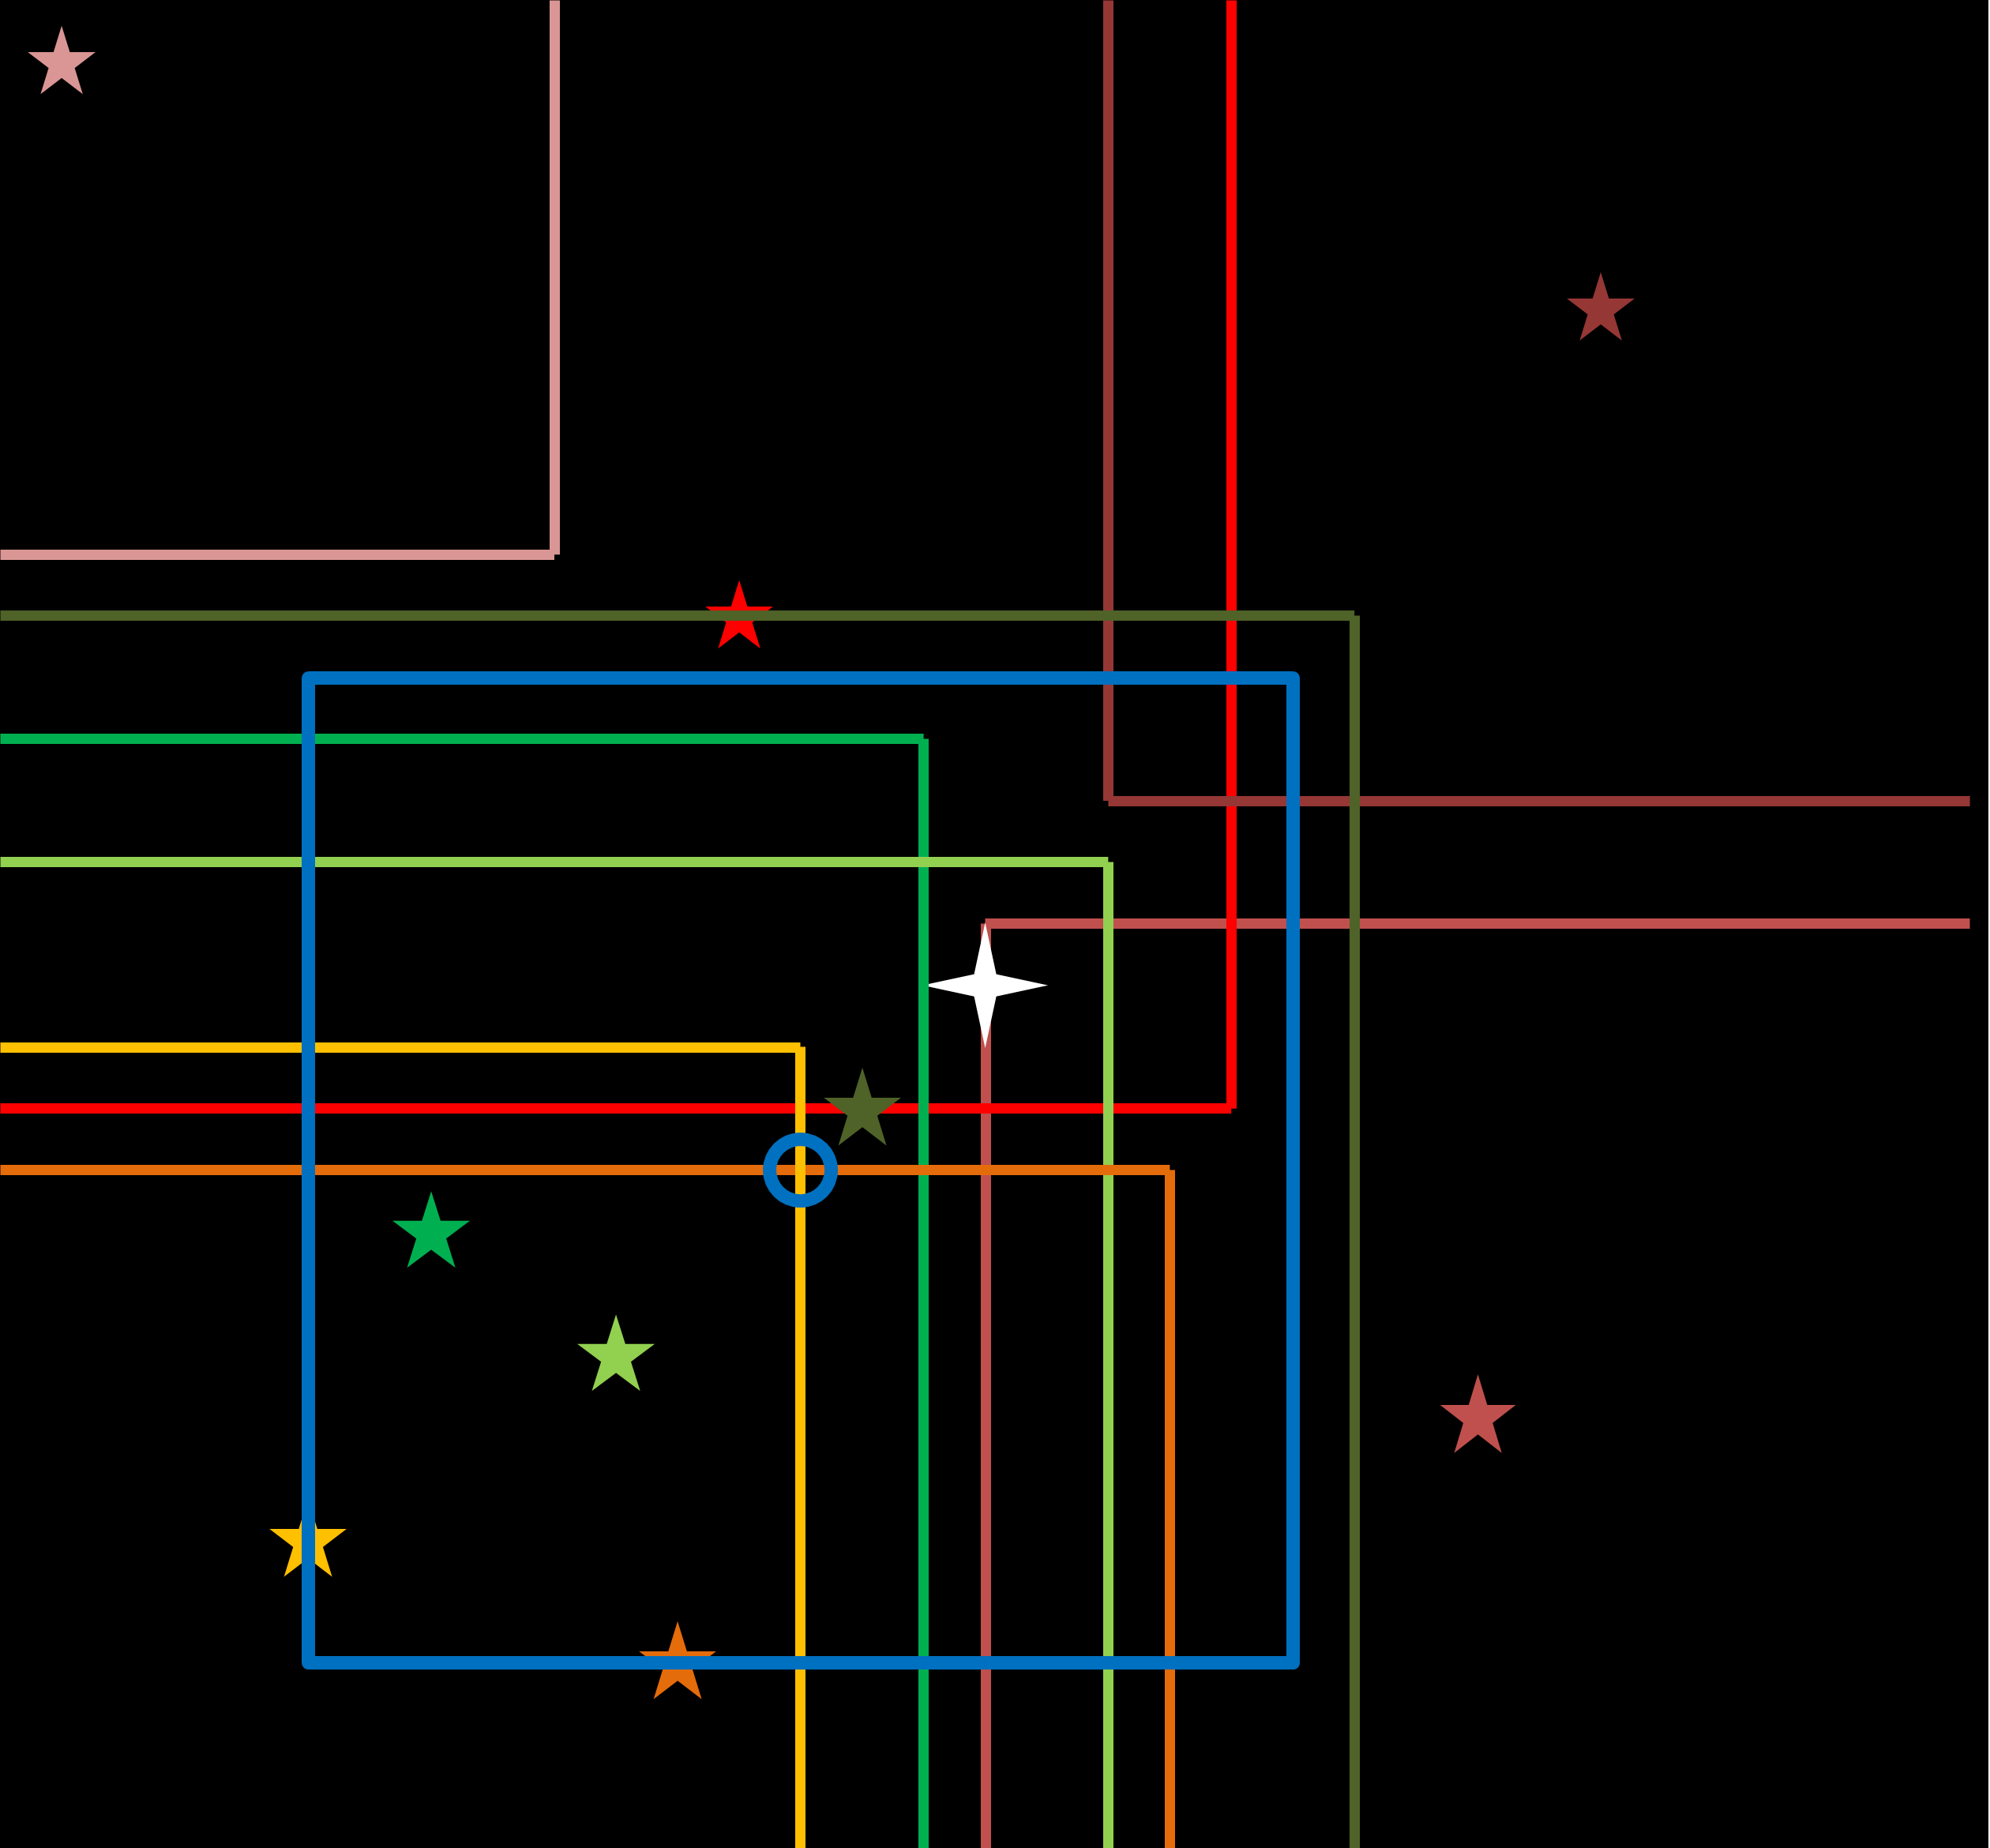
\includegraphics{fig5.png}
\caption{Figure 5: Locus Algorithm. Target: white star. Pointing \& FoV:
blue. Reference stars and their loci: Fully in the FoV: greens. On the
edge of the FoV: yellows. Outside FoV: reds}
\end{figure}

\newpage

Scenarios can arise which result in an inability to identify an optimum
pointing for a given target for example if there are no, or a maximum of
one reference stars in the candidate zone; and if no points of
intersection arise -- a scenario which can arise if two (or more)
reference fall in one quadrant of the candidate zone resulting in
concentric loci, or where reference stars are too far apart in different
quadrants of the candidate zone in order for their loci to intersect.
All four of these scenarios are considered in practical implementations
of the locus algorithm aimed at identifying the optimum pointings for a
set of targets in a catalogue or list of targets.

In summary, the Locus Algorithm successfully identifies the RA and Dec
coordinates of the optimum pointing for a given target, where optimum
means a field of view with the maximum number of reference stars which
are similar in magnitude and colour to the target.

\newpage

\hypertarget{example-implementation-of-the-locus-algorithm}{%
\section{Example Implementation of the Locus
Algorithm}\label{example-implementation-of-the-locus-algorithm}}

To illustrate the operations of the Locus Algorithm, a worked example is
given here. The process described here in producing an optimal pointing
for a given star follows the same sequence of steps described in the
first part of this paper. The process is implemented in the R
programming language and is geared for reproducible research. The code
is available on
\emph{\textbf{\href{https://github.com/eugene100hickey/LocusAlgorithm}{github}}}.
It can be trivially adapted for different target stars and telescope
parameters.

\hypertarget{target}{%
\subsection{Target}\label{target}}

The star with SDSS ID 1237680117417115655, henceforth called the target,
(RA = 346.65 and DEC = -5.0393) is used as the example. This star, in
the constellation Aquarius, has SDSS magnitudes as given in the table
below. \vskip 0.2in

\begin{table}[H]
\centering
\begin{tabular}{l|r}
\hline
Band & SDSS\_Magnitude\\
\hline
u & 17.20\\
\hline
g & 15.38\\
\hline
r & 14.65\\
\hline
i & 14.40\\
\hline
z & 14.28\\
\hline
\end{tabular}
\end{table}

The observational parameters are taken from the telescope at
\href{www.bco.ie}{Blackrock Castle Observatory}. This telescope has
parameters given in the table below: \vskip 0.2in

\begin{table}[H]
\centering
\begin{tabular}{l|r}
\hline
Parameters & Values\\
\hline
Field of View in degrees & 0.1667\\
\hline
Resolution Limit in degrees & 0.0030\\
\hline
Dynamic Range in magnitudes & 2.0000\\
\hline
Colour Match Limit & 0.1000\\
\hline
\end{tabular}
\end{table}

\hypertarget{candidate-zone-1}{%
\subsection{Candidate Zone}\label{candidate-zone-1}}

The size of the FoV when corrected for shortening by declination is, by
equation 1 above,

\[R^` = {\frac{R}{cos(Dec_c)}}\]

\center = 0.1667 / cos(-5.0393 \(^{\circ}\)) \center

\center = 0.16731 \(^{\circ}\) \center

The locus of the target is, by equation 2 above,

\center 346.5664 \(\leq\) RA \(\leq\) 346.7337 \center \center -5.1226
\(\leq\) Dec \(\leq\) -4.956 \center

The candidate zone as defined above is the area of sky within which
reference stars can possibly be included in the same field of view as
the target. This is four times the size of the FoV and is given by
equation 3 above,

\center 346.4827 \(\leq\) RA \(\leq\) 346.8173 \center \center -5.206
\(\leq\) Dec \(\leq\) -4.8726 \center

\newpage

\hypertarget{identification-and-filtering-of-reference-stars-1}{%
\subsection{Identification and Filtering of Reference
Stars}\label{identification-and-filtering-of-reference-stars-1}}

The potential reference stars are selected as follows:

\begin{itemize}
\tightlist
\item
  Position: Within the Candidate Zone, SDSS records 1345 separate
  objects with clean photometry, (Aguado et al. (2018)).
\item
  Magnitude: the reference star must be within the dynamic range, 2, of
  the target's magnitude of 14.648, e.g.~12.648 \(\leq\) r \(\leq\)
  16.648. This leaves 41 potential references.
\item
  Colour: the reference star must match the colour of the target to
  within a user-specified limit. In this case this means \(g - r\)
  between 0.634 and 0.834 and \(r - i\) between 0.149 and 0.349 This
  leaves 15 potential references.
\item
  Resolvability: the reference star must be resolvable, i.e.~no other
  star that would impact a brightness measurements within a
  user-specified resolution limit, in this case 11 arc seconds, (0.18
  arc minutes). Any object this close to a potential reference star and
  with an r-band magnitude which is 5 magnitudes greater than the
  potential reference or brighter will pollute the light from the
  potential reference star. This leaves 14 potential references.
\end{itemize}

These numbers are presented in the table below. \vskip 0.2in

\begin{table}[H]
\centering
\begin{tabular}{l|r}
\hline
filters & numbers\\
\hline
Position, in Field of View & 1345\\
\hline
Correct Magnitude & 41\\
\hline
Correct Colour & 15\\
\hline
Resolvable & 14\\
\hline
In Final Field of View & 7\\
\hline
\end{tabular}
\end{table}

\vskip 0.2in

The table below gives the 14 stars in the candidate zone along with the
highlighted 7 stars in the final field of view.

\vskip 0.2in

\begin{table}[H]
\centering
\begin{tabular}{l|l|r|r|r|r|r|r|r|r}
\hline
ref. & objID & ra & dec & mag\_u & mag\_g & mag\_r & mag\_i & mag\_z & ratings\\
\hline
1 & 1237680117417115701 & 346.743 & -5.005 & 18.461 & 16.409 & 15.583 & 15.317 & 15.160 & 0.068\\
\hline
\rowcolor[HTML]{D7261E}  \textcolor{white}{\textbf{2}} & \textcolor{white}{\textbf{1237680117417050133}} & \textcolor{white}{\textbf{346.594}} & \textcolor{white}{\textbf{-5.161}} & \textcolor{white}{\textbf{16.702}} & \textcolor{white}{\textbf{14.825}} & \textcolor{white}{\textbf{14.068}} & \textcolor{white}{\textbf{13.887}} & \textcolor{white}{\textbf{13.648}} & \textcolor{white}{\textbf{0.241}}\\
\hline
3 & 1237680065885306903 & 346.669 & -4.915 & 17.716 & 15.654 & 14.897 & 14.691 & 14.450 & 0.429\\
\hline
4 & 1237680117417050117 & 346.538 & -5.018 & 18.404 & 16.520 & 15.768 & 15.532 & 15.393 & 0.701\\
\hline
\rowcolor[HTML]{D7261E}  \textcolor{white}{\textbf{5}} & \textcolor{white}{\textbf{1237680065348435996}} & \textcolor{white}{\textbf{346.707}} & \textcolor{white}{\textbf{-5.199}} & \textcolor{white}{\textbf{16.704}} & \textcolor{white}{\textbf{14.699}} & \textcolor{white}{\textbf{13.905}} & \textcolor{white}{\textbf{13.676}} & \textcolor{white}{\textbf{13.515}} & \textcolor{white}{\textbf{0.322}}\\
\hline
6 & 1237680065885241371 & 346.560 & -4.931 & 17.680 & 15.934 & 15.227 & 15.012 & 14.901 & 0.485\\
\hline
\rowcolor[HTML]{D7261E}  \textcolor{white}{\textbf{7}} & \textcolor{white}{\textbf{1237680117417115683}} & \textcolor{white}{\textbf{346.713}} & \textcolor{white}{\textbf{-5.050}} & \textcolor{white}{\textbf{17.585}} & \textcolor{white}{\textbf{15.782}} & \textcolor{white}{\textbf{15.109}} & \textcolor{white}{\textbf{14.867}} & \textcolor{white}{\textbf{14.798}} & \textcolor{white}{\textbf{0.361}}\\
\hline
9 & 1237680065885241391 & 346.483 & -4.946 & 18.969 & 17.144 & 16.420 & 16.161 & 15.991 & 0.808\\
\hline
\rowcolor[HTML]{D7261E}  \textcolor{white}{\textbf{10}} & \textcolor{white}{\textbf{1237680117417050120}} & \textcolor{white}{\textbf{346.563}} & \textcolor{white}{\textbf{-5.153}} & \textcolor{white}{\textbf{18.460}} & \textcolor{white}{\textbf{16.498}} & \textcolor{white}{\textbf{15.771}} & \textcolor{white}{\textbf{15.533}} & \textcolor{white}{\textbf{15.397}} & \textcolor{white}{\textbf{0.830}}\\
\hline
\rowcolor[HTML]{D7261E}  \textcolor{white}{\textbf{11}} & \textcolor{white}{\textbf{1237680117417115692}} & \textcolor{white}{\textbf{346.724}} & \textcolor{white}{\textbf{-5.047}} & \textcolor{white}{\textbf{18.362}} & \textcolor{white}{\textbf{16.576}} & \textcolor{white}{\textbf{15.843}} & \textcolor{white}{\textbf{15.568}} & \textcolor{white}{\textbf{15.464}} & \textcolor{white}{\textbf{0.734}}\\
\hline
\rowcolor[HTML]{D7261E}  \textcolor{white}{\textbf{12}} & \textcolor{white}{\textbf{1237680117417115762}} & \textcolor{white}{\textbf{346.676}} & \textcolor{white}{\textbf{-5.120}} & \textcolor{white}{\textbf{18.920}} & \textcolor{white}{\textbf{17.022}} & \textcolor{white}{\textbf{16.282}} & \textcolor{white}{\textbf{15.974}} & \textcolor{white}{\textbf{15.851}} & \textcolor{white}{\textbf{0.380}}\\
\hline
13 & 1237680065348501526 & 346.804 & -5.202 & 15.877 & 14.146 & 13.385 & 13.148 & 12.994 & 0.644\\
\hline
\rowcolor[HTML]{D7261E}  \textcolor{white}{\textbf{14}} & \textcolor{white}{\textbf{1237680117417115655}} & \textcolor{white}{\textbf{346.650}} & \textcolor{white}{\textbf{-5.039}} & \textcolor{white}{\textbf{17.199}} & \textcolor{white}{\textbf{15.382}} & \textcolor{white}{\textbf{14.648}} & \textcolor{white}{\textbf{14.399}} & \textcolor{white}{\textbf{14.281}} & \textcolor{white}{\textbf{1.000}}\\
\hline
15 & 1237680117417181202 & 346.810 & -4.975 & 17.461 & 15.616 & 14.852 & 14.579 & 14.443 & 0.535\\
\hline
\end{tabular}
\end{table}

The table above also includes ratings for each star. This gives a
measure of how close, spectrally, each reference star is to the target.
This rating hasn't been optimised and is the subject of further research
by our group, but for the purpose of this work was calculated as
follows:

\[rating = \abs{(1-\frac{\delta g - \delta r}{M})} \times \abs{(1-\frac{\delta r - \delta i}{M})}\]

Where \(\delta r\) stand for the difference between the r-band magnitude
for the target and the reference star and M is the colour match limit.
Similarly for \(\delta g\) and \(\delta i\).

For example, the star SDSS1237680117417050120 (Star 10 on figure N) has
g\(_r\) = 16.498, r\(_r\) = 15.771, and i\(_r\) = 15.533. This compares
to the target magnitudes of g\(_t\) = 15.382, r\(_t\) = 14.648, and
i\(_t\) = 14.399.

This gives: \(\delta g\) = 16.498 - 15.382 = 1.116. \(\delta r\) =
15.771 - 14.648 = 1.122. \(\delta i\) = 15.533 - 14.399 = 1.134. Thus
rating = (1 - (\textbar{}1.116 - 1.122)/0.1\textbar{}) \(\times\) (1 -
(\textbar{}1.122 - 1.134)/0.1\textbar{}) = (0.93) \(\times\) (0.89)

= 0.83

\newpage

From expression 8, the cornerpoints for a given reference can be
calculated: \[RA_r < RA_t => RA_c = RA_r + R'\]

\[Dec_r < Dec_t => Dec_c = Dec_r + S\]

For reference SDSS1237680117417050120 (Star 10 on figure N) \vskip 0.2in
346.5626 \textless{} 346.65 =\textgreater{} RA\textsubscript{c} =
346.5626 + 0.0837 = 346.6463 \vskip 0.2in -5.153 \textless{} -5.0393
=\textgreater{} Dec\textsubscript{c} = -5.153 + 0.0833 = -5.0697

From Expression 9: RA\textsubscript{r} \textless{} RA\textsubscript{t}
=\textgreater{} DirRA = +ive Dec\textsubscript{r} \textless{}
Dec\textsubscript{t} =\textgreater{} DirDec = +ive \vskip 0.2in For
reference SDSS1237680117417050120 (Star 10 on figure N) \vskip 0.2in
346.5626 \textless{} 346.65 =\textgreater{} DirDec = +ive,\\
-5.153 \textless{} -5.0393 =\textgreater{} DirRA = +ive \vskip 0.2in
Repeating this calculation for SDSS1237680065348435996 (Star 5 on figure
N) gives RA\textsubscript{c} = 346.6235, Dec\textsubscript{c} = -5.1153,
\vskip 0.2in DirRA = -ive, DirDec = +ive.

We can compare these two effective loci to see if they intersect to form
a valid PoI. \vskip 0.2in From Expression 10: DirRA10 = +ive,
DirDec5=-ive RA\textsubscript{r}10 \textless{} RA\textsubscript{r}5 AND
Dec\textsubscript{r}10 \textgreater{} Dec\textsubscript{r}5

PoI exist at (RA\textsubscript{c}10, Dec\textsubscript{c}10) =
(346.6463, -5.1153) \vskip 0.2in From Expression 2, the FoV centred on
the PoI (346.6463, -5.1153) can be calculated to be:

\[RA_c - {\frac{R^`}{2}} \leq RA \leq RA_c + {\frac{R^`}{2}} \]

\[Dec_c - {\frac{S}{2}} \leq Dec \leq Dec_c + {\frac{S}{2}}\]

346.6463 - 0.0837 \(\leq\) RA \(\leq\) 346.6463 + 0.0837 \vskip 0.2in
-5.1153 - 0.0833 \(\leq\) Dec \(\leq\) -5.1153 + 0.0833 \vskip 0.2in
346.5626 \(\leq\) RA \(\leq\) 346.7299 \vskip 0.2in -5.1987 \(\leq\) Dec
\(\leq\) -5.032 \newpage

The locus associated with each of these 14 potential references is
identified and the Points of Intersection associated with these locii
are calculated. This leads to the situation shown in the diagram below

\includegraphics{Locus_Whole_files/figure-latex/candidate_plot-1.pdf}

After checking different fields of view, a pointing with RA = 346.646
and DEC = -5.115 included both the target and 7 reference stars. This
pointing is calculated to have a score of 3.87 \newpage

The SQL query to download potential reference stars from SDSS is given
below. This SQL query is run on the CAS database, release DR15, of SDSS.
Note the flags to give clean photometry (Aguado et al. (2018))
\vskip 0.2in \noindent SELECT objID, ra, dec, psfmag\_u, psfmag\_g,
psfmag\_r, psfmag\_i, psfmag\_z

FROM photoObj

WHERE (ra between (346.48270496969) AND (346.817331746246)

OR ra BETWEEN (706.48270496969) AND (706.817331746246)

OR ra BETWEEN (-13.5172950303096) AND (-13.1826682537544) ) AND dec
BETWEEN (-5.20597532982638) AND (-4.87264199649304)

AND psfmag\_r BETWEEN 12.64849 AND 16.64849

AND (psfmag\_g - psfmag\_r) BETWEEN (0.633989999999999) AND
(0.833989999999999)

AND (psfmag\_r - psfmag\_i) BETWEEN (0.149080000000001) AND
(0.349080000000001)

AND clean = 1

AND (calibStatus\_r \& 1) != 0 \vskip 0.2in

\begin{tabular}{l|l|r|r|r|r|r|r|r|r}
\hline
ref. & objID & ra & dec & mag\_u & mag\_g & mag\_r & mag\_i & mag\_z & ratings\\
\hline
10 & 1237680117417050120 & 346.563 & -5.153 & 18.460 & 16.498 & 15.771 & 15.533 & 15.397 & 0.830\\
\hline
2 & 1237680117417050133 & 346.594 & -5.161 & 16.702 & 14.825 & 14.068 & 13.887 & 13.648 & 0.241\\
\hline
14 & 1237680117417115655 & 346.650 & -5.039 & 17.199 & 15.382 & 14.648 & 14.399 & 14.281 & 1.000\\
\hline
12 & 1237680117417115762 & 346.676 & -5.120 & 18.920 & 17.022 & 16.282 & 15.974 & 15.851 & 0.380\\
\hline
5 & 1237680065348435996 & 346.707 & -5.199 & 16.704 & 14.699 & 13.905 & 13.676 & 13.515 & 0.322\\
\hline
7 & 1237680117417115683 & 346.713 & -5.050 & 17.585 & 15.782 & 15.109 & 14.867 & 14.798 & 0.361\\
\hline
11 & 1237680117417115692 & 346.724 & -5.047 & 18.362 & 16.576 & 15.843 & 15.568 & 15.464 & 0.734\\
\hline
\end{tabular}

\includegraphics{Locus_Whole_files/figure-latex/locus_plot-1.pdf}

\newpage

\hypertarget{references}{%
\subsection*{References}\label{references}}
\addcontentsline{toc}{subsection}{References}

\hypertarget{refs}{}
\leavevmode\hypertarget{ref-Aguado2018}{}%
Aguado, D. S., Romina Ahumada, Andres Almeida, Scott F. Anderson, Brett
H. Andrews, Borja Anguiano, Erik Aquino Ortiz, et al. 2018. ``The
Fifteenth Data Release of the Sloan Digital Sky Surveys: First Release
of MaNGA Derived Quantities, Data Visualization Tools and Stellar
Library,'' December. \url{https://doi.org/10.3847/1538-4365/aaf651}.

\leavevmode\hypertarget{ref-Honeycutt1992}{}%
Honeycutt, R. K. 1992. ``CCD ensemble photometry on an inhomogeneous set
of exposures.'' \emph{Publications of the Astronomical Society of the
Pacific} 104 (676). IOP Publishing: 435.
\url{https://doi.org/10.1086/133015}.

\leavevmode\hypertarget{ref-Howell2000}{}%
Howell, Steve B., and Steve B. 2000. ``Handbook of CCD Astronomy.''
\emph{Handbook of CCD Astronomy / Steve B. Howell. Cambridge, U.K. ; New
York : Cambridge University Press, C2000. (Cambridge Observing Handbooks
for Research Astronomers ; 2)}.
\url{http://adsabs.harvard.edu/abs/2000hccd.book.....H}.

\leavevmode\hypertarget{ref-Milone2011}{}%
Milone, E. F., and Jan Willem Pel. 2011. ``The High Road to Astronomical
Photometric Precision: Differential Photometry.'' In \emph{Astronomical
Photometry: Past, Present, and Future, Edited by E.f. Milone and c.
Sterken. Astrophysics and Space Science Library, Vol. 373. Berlin:
Springer, 2011. ISBN 978-1-4419-8049-6, P. 33-68}, 373:33--68.
\url{https://doi.org/10.1007/978-1-4419-8050-2_2}.

\leavevmode\hypertarget{ref-YOUNG1991}{}%
YOUNG, ANDREW T., RUSSELL M. GENET, LOUIS J. BOYD, WILLIAM J. BORUCKI,
G. WESLEY LOCKWOOD, GREGORY W. HENRY, DOUGLAS S. HALL, et al. 1991.
``PRECISE AUTOMATIC DIFFERENTIAL STELLAR PHOTOMETRY.'' Astronomical
Society of the Pacific. \url{https://doi.org/10.2307/40679676}.

\end{document}


